\documentclass[10pt]{article}
\makeatletter
\usepackage{lmodern}
\usepackage{comment}
\excludecomment{Answ}
\usepackage{listings}
\usepackage{color} %red, green, blue, yellow, cyan, magenta, black, white
\definecolor{mygreen}{RGB}{28,172,0} % color values Red, Green, Blue
\definecolor{mylilas}{RGB}{170,55,241}
\renewcommand\paragraph{\@startsection{paragraph}{4}{\z@}%
            {-2.5ex\@plus -1ex \@minus -.25ex}%
            {1.25ex \@plus .25ex}%
            {\normalfont\normalsize\bfseries}}
\makeatother
\usepackage{gensymb}
\setcounter{secnumdepth}{4}
\usepackage{amsmath}
%\usepackage{mathtools}
\usepackage{graphicx}
\usepackage{slashed}
\usepackage{lineno}
\usepackage{latexsym}
\usepackage{subfigure}
\usepackage{amssymb}
\newtheorem{thm}{Theorem}[section]
\newtheorem{cor}[thm]{Corollary}
\newtheorem{lem}[thm]{Lemma}
\usepackage[numbers,sort]{natbib}
\usepackage{enumerate}
\newcommand{\bb}{\begin{equation}}
\newcommand{\ee}{\end{equation}}
\newtheorem{defin}{Definition}
\usepackage{multirow}
\usepackage{ctable}
\usepackage{bm}
\usepackage{enumerate}
\newcommand{\D}[2]{\frac{\partial #1}{\partial #2}}
\newcommand{\DD}[2]{\frac{\partial^2 #1}{\partial #2^2}}
\newcommand{\rd}{\text{ d}}
\newcommand{\disk}{}
\usepackage{framed}
\newcommand{\see}[1]{(see Figure \ref{#1})}
\newcommand{\fig}[1]{Figure \ref{#1}}
\newcommand{\figs}[2]{figures \ref{#1} and \ref{#2}}
\newcommand{\sect}[1]{Section \ref{#1}}
\newcommand{\app}[1]{Appendix \ref{#1}}
\newcommand{\chap}[1]{Chapter \ref{#1}}
\newcommand{\eqn}[1]{equation \eqref{#1}}
\newcommand{\eqns}[2]{equations \eqref{#1} and \eqref{#2}}
\newcommand{\eqnto}[2]{equations \eqref{#1}-\eqref{#2}}
%\usepackage{authblk}
\usepackage{url}
\usepackage{soul}
\newcommand{\eg}{\emph{e.g.} }
\newcommand{\bn}{\bm{n}}
\newcommand{\bu}{\bm{u}}
\newcommand{\ie}{\emph{i.e.} }
\newcommand{\Chapter}[1]{\chapter{#1}\label{#1}}
\newcommand{\Section}[1]{\section{#1}\label{#1}}
\newcommand{\Subsection}[1]{\subsection{#1}\label{#1}}
\newcommand{\Subsubsection}[1]{\subsubsection{#1}\label{#1}}
\newcommand{\Appendix}[1]{\appendix{#1}\label{#1}}
\usepackage[margin=1.5cm,centering]{geometry}
\usepackage[geometry]{ifsym}
\makeatletter
\newcommand\restr[2]{{% we make the whole thing an ordinary symbol
  \left.\kern-\nulldelimiterspace % automatically resize the bar with \right
  #1 % the function
  \vphantom{\big|} % pretend it's a little taller at normal size
  \right|_{#2} % this is the delimiter
  }}
\def\url@leostyle{%
  \@ifundefined{selectfont}{\def\UrlFont{\sf}}{\def\UrlFont{\small\ttfamily}}}
\makeatother
\urlstyle{leo}
\usepackage{multirow}
\usepackage{blkarray}
\usepackage{soul}
\usepackage{framed}
\usepackage{color}
\usepackage{setspace}
\newcommand{\ttttp}{.24\textwidth}
\newcommand{\tttp}{.32\textwidth}
\newcommand{\ttp}{.45\textwidth}
\newcommand{\tbo}{.6\textwidth}
 \usepackage[T1]{fontenc}
\usepackage[utf8]{inputenc}
\usepackage{authblk}
 \renewcommand{\l}{\left(}
\renewcommand{\r}{\right)}
%\begin{figure}[h!!!tb]
%\centering
%\subfigure[\label{Godzilla}]{\includegraphics[height=0.35\textwidth]{./Pictures/Godzilla_final_bw.png}}
%\subfigure[\label{Jaeger}]{\includegraphics[height=0.35\textwidth]{./Pictures/Jaeger_finish_bw.png}}
%\caption{\label{Monsters} The two types of monster we are going to consider are: (a) the naturally occurring Kaijus and (b) the man-made Jaegers.}
%\end{figure}


\begin{document}

\lstset{language=Matlab,%
    %basicstyle=\color{red},
    breaklines=true,%
    morekeywords={matlab2tikz},
    keywordstyle=\color{blue},%
    morekeywords=[2]{1}, keywordstyle=[2]{\color{black}},
    identifierstyle=\color{black},%
    stringstyle=\color{mylilas},
    commentstyle=\color{mygreen},%
    showstringspaces=false,%without this there will be a symbol in the places where there is a space
    numbers=left,%
    numberstyle={\tiny \color{black}},% size of the numbers
    numbersep=9pt, % this defines how far the numbers are from the text
    emph=[1]{for,end,break},emphstyle=[1]\color{red}, %some words to emphasise
    %emph=[2]{word1,word2}, emphstyle=[2]{style},    
}


\title{Problem sheet 1}
\author{Thomas E. Woolley\\Last edited on:}
\maketitle
\section{Carbon dating}

Radioactive carbon-14 in the atmosphere combines with oxygen to form carbon dioxide. This carbon dioxide is ingested by plants, which in turn are eaten by animals. In
this way all living plants and animals absorb quantities of radioactive carbon-14.

When a plant or animal dies, the carbon-14 in the tissue begins to decay. Thus, the age of an artefact that contains plant or animal material can be estimated by determining what percentage of its original carbon-14 content remains.

The carbon-14 content of organic matter decays exponentially. Thus, the percentage, $p$, of carbon-14 in an artefact is defined by
\bb
\dot{p}=-0.000121p,\quad p(0)=100\%,\label{Carbon_decay}
\ee
where 0.000121/year is the decay constant for carbon-14.

In 1988 the Vatican authorized the British Museum to date a cloth relic known as the Shroud of Turin \see{Turing_shroud}. This cloth, which first surfaced in 1356, contains the negative image of a human body that was widely believed to be that of Jesus. The report of the British Museum showed that the fibres in the cloth contained between 92\% and 93\% of their original carbon-14.
\begin{enumerate}
\item Use the above information to estimate the age of the shroud.
\item State an assumption that has been made which will cause the answer to be incorrect.
\end{enumerate}
\begin{figure}[h!!!tb]
\centering
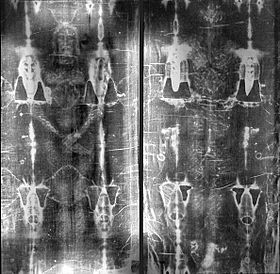
\includegraphics[width=0.4\textwidth]{../../Pictures/Turin_shroud.jpg}
\caption{\label{Turing_shroud} The Turin Shroud.}
\end{figure}
\begin{Answ}
\subsection{Answers}
\subsubsection{}
Solving \eqn{Carbon_decay} gives the following equation for the fraction of the original carbon-14 that remains after $t$ years:
\bb
p(t)=100\exp(-0.000121 t).
\ee
Taking the natural logarithm of both sides and solving for $t$, we obtain
\bb
t = -\frac{1}{0.000121}\log\l \frac{p(t)}{100}\r.
\ee
Substituting $p(t)$ for 92\% or 93\% puts the age of the shroud between 600 and 689 years old. Since the test was done in 1988, the shroud originates between 1299 A.D. and 1388 A.D. Thus, if one accepts the validity of carbon-14 dating, the Shroud of Turin cannot be the burial shroud of Jesus.
\subsubsection{}
We are assuming that:
\begin{itemize}
\item the rate of decay of carbon-14 is constant throughout history.
\item the proportion estimated by the British Museum assumes that that the amount taken up by organic matter is a constant.
\item other assumptions are possible.
\end{itemize}
\end{Answ}
\section{Hinged door}
Fire doors are usually attached to damped spring hinges so that they cause a door to return to a closed position, rather than stay open. The position, $y$, of the door can be modelled as a damped oscillator, where the damping is proportional to the door's speed, $\dot{y}$,
\bb
\underbrace{\ddot{y}=-ky}_{\textrm{Simple harmonic motion}}-\underbrace{a\dot{y},}_{\textrm{Motion damping}}\quad y(0)=y_0, \dot{y}(0)=0.\label{Damped}
\ee
where $k$ and $a$ are positive constants.
\begin{enumerate}
\item Substitute the solution form $y(t)=A\exp(\lambda t)$ into \eqn{Damped}. What values must $\lambda$ take in order for this solution to exist?
\item Describe the solutions you get in the two different cases
\bb
\textrm{(i)} \l\frac{a}{2}\r^2>k,\quad\quad \textrm{(ii)} \l\frac{a}{2}\r^2<k.
\ee
\item Which case is preferential for a fire door?
\end{enumerate}
\begin{Answ}
\subsection{Answers}
\subsubsection{}
Substituting $y(t)=A\exp(\lambda t)$ into \eqn{Damped} and simplifying provides us with the auxiliary equation
\bb
\lambda^2+a\lambda+k=0.
\ee
This has solution
\bb
\lambda_\pm=\frac{-a\pm\sqrt{a^2-4k}}{2}.
\ee
\subsubsection{}
If $\l a/2\r^2>k$ then both roots of $\lambda_\pm$ are real. Moreover, since the constants are all positive we know that $\lambda_-<\lambda_+<0$. Hence, the position of the door will follow a negative exponential. This is called over damping.

If $\l a/2\r^2<k$ then both roots of $\lambda_\pm$ are imaginary. We split the exponential solution form into its real and negative parts and use the trigonometric identity,
\bb
\exp\l-\frac{at}{2}\r\exp\l\frac{It\sqrt{4k-a^2}}{2}\r=\exp\l-\frac{at}{2}\r\l\cos\l t\frac{\sqrt{4k-a^2}}{2}\r+I\sin\l t\frac{\sqrt{4k-a^2}}{2}\r\r.
\ee
Since $a>0$ and the trig functions are bounded this solution also tends to zero, but the trigonometric component causes the door to oscillate. This in called under damping.

\subsubsection{}
We want fire doors to be over damped because we do not want them to oscillate after they have been released. Specifically, this protects anyone approaching the door after us (\ie they will not get hit in the face) and means that if there is a fire then the door will close immediately and not let further oxygen in to feed the flames.
\end{Answ}
\section{Motion under gravity}
In the 1994 film True Lies a terrorist uses a motorbike to jump off of one building onto another. Arnold Schwarzenegger then tries to follow the terrorist on a horse. However, the horse thinks better of this and stops before jumping (see the clip for yourself http://bit.ly/2lf1HgL). Here are some facts to digest:
\begin{itemize}
\item The hotel in the film is The Westin Bonaventure Hotel. 
\item The pool the terrorist lands in is 85m away (horizontally) and 100m below \see{True_lies}.
\item The motorbike is a Kawasaki EX500.
\item The bike has a run up of 13m along the hotel roof.
\item The bike has a maximum acceleration of 0-60 mph in 3.76 sec.
\item A trained racehorse has a maximum acceleration of 13.4 m/s$^2$.
\item The acceleration rate due to gravity is 9.81m/s$^2$.
\item The horse and rider weigh 700kg.
\end{itemize}
Using the knowledge that acceleration, $a$, is the rate of change of velocity, $v$, over time and velocity is the rate of change of displacement, $x$, over time, \ie
\bb
a=\dot{v}=\ddot{x},
\ee
solve the following questions.
\begin{figure}[h!!!tb]
\centering
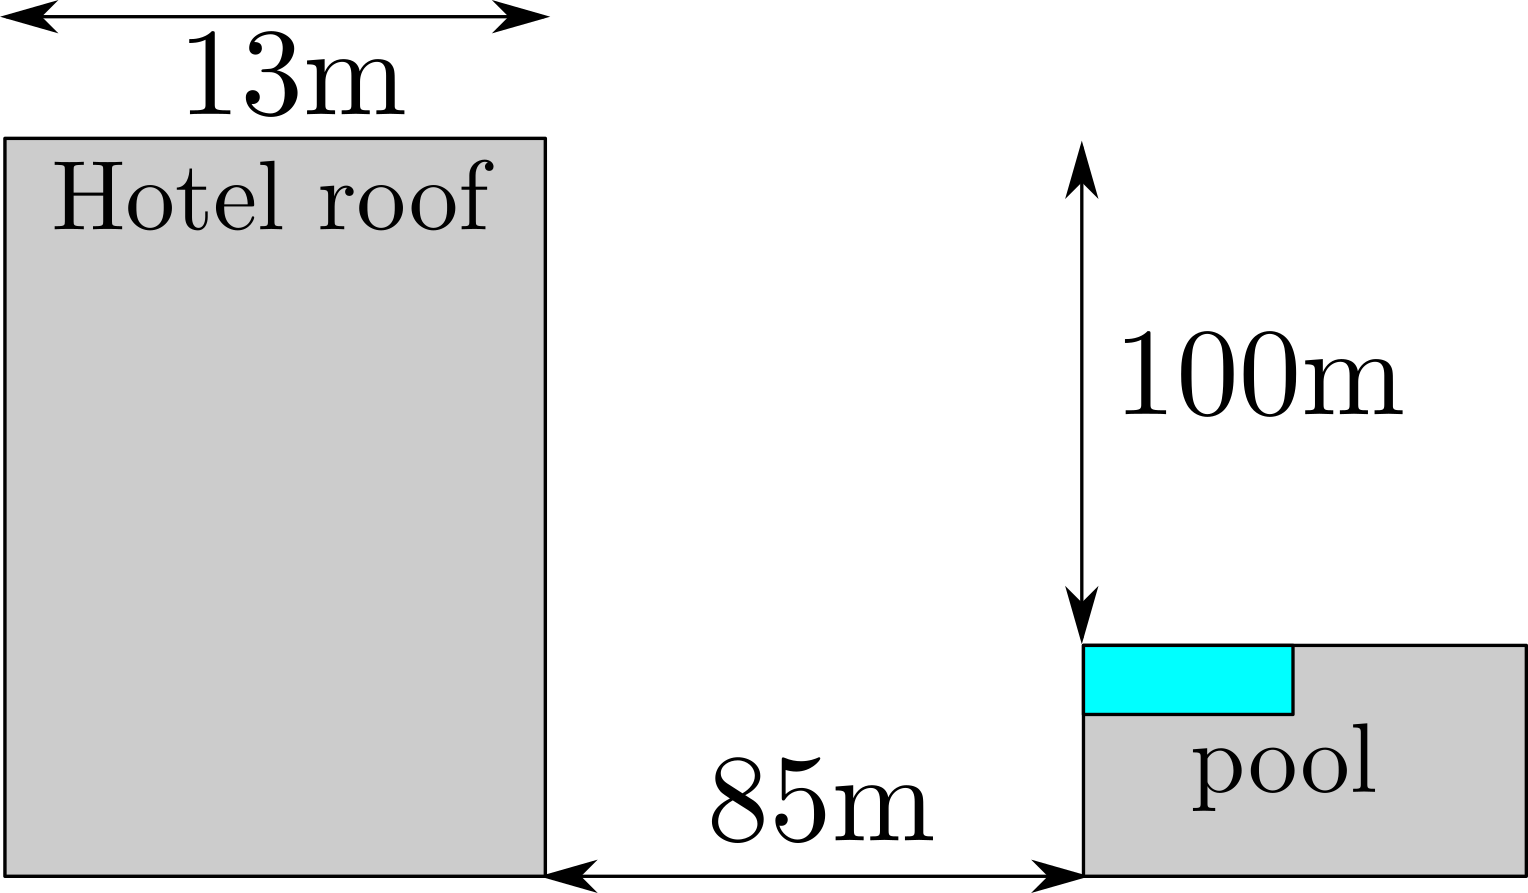
\includegraphics[width=0.4\textwidth]{../../Pictures/True_lies.png}
\caption{\label{True_lies} Schematic of the jump from True lies. Not to scale.}
\end{figure}
\begin{enumerate}
\item Assuming the bike has constant acceleration over time, use the data to determine the maximum acceleration of the bike in m/s$^2$? Hint: the linear acceleration is calculated by change in speed divided by time taken.
\item The acceleration in the $x$ and $y$ directions is $\ddot{x}$ and $\ddot{y}$, namely the second derivative of the coordinate with respect to time. Assuming the bike was initially stationary and the acceleration was constant over the 13m of the flat hotel roof, how fast is the bike going (horizontally and vertically) at the moment it leaves the roof top?\label{Vel}
\item At the moment the bike leaves the roof top, what is the acceleration in the horizontal and vertical directions? \label{acc}
\item Using the equations from question \ref{acc} and the values from point \ref{Vel} as initial data, how long does it take the bike to fall 100m? How far could the bike travel horizontally in that time? Could the motorbike have made the jump?
\item Could the horse have made the jump?
\item What have you assumed? Would altering these assumptions qualitatively change the results of the question?
\end{enumerate}
\begin{Answ}
\subsection{Answers}
\subsubsection{}
The bike's speed increases to 60mph=26.8m/s over 3.76 seconds, thus acceleration is $a=26.8/3.76=7.13$m/s$^2$.
\subsubsection{}
Integrating the relationship we have that $v=7.13t$ and $x=7.13t^2/2$. Rearranging, we get $v=7.13\sqrt{2x/7.13}$. Substituting $x=13$ into this equation we get $v=13.6$m/s. Thus, at the moment the bike leaves the hotel roof the horizontal component of the velocity will be 13.6m/s. The vertical component will be 0m/s
\subsubsection{}
We consider the displacement, velocity and acceleration is both vertical and horizontal directions
\bb
\left(
\begin{array}{c}
\ddot{x}\\
\ddot{y}\\
\end{array}
\right)=\left(
\begin{array}{c}
0\\
-9.81\\
\end{array}
\right).
\ee
\subsubsection{}
Through integration we derive
\bb
\left(
\begin{array}{c}
\dot{x}\\
\dot{y}\\
\end{array}
\right)=\left(
\begin{array}{c}
13.6\\
-9.81t\\
\end{array}
\right), \quad \left(
\begin{array}{c}
x\\
y\\
\end{array}
\right)=\left(
\begin{array}{c}
13.6t\\
-\frac{9.81}{2}t^2\\
\end{array}
\right).
\ee
Using the equation for $y$ we can calculate the time to fall 100m as $t=\sqrt{100\times 2/9.81}=4.52$s. This can be substituted into the horizontal displacement equation, $x=13.6 \times 4.52=61.4$m. Thus, the motorbike could not have made the jump.
\subsubsection{}
Rerunning the questions with a horse acceleration of 13.4m/s$^2$, gives
\bb
v=13.4\sqrt{2x/13.4}=18.7\textrm{m/s}.
\ee
The horse will take the same time, $t=4.52$, to drop 100m. In this time the horse will travel $x=18.7\times 4.52=84.4$m. The horse just misses the pool.
\subsubsection{}
We have assumed:
\begin{itemize}
\item no air resistance;
\item constant acceleration;
\item that the horse is a racehorse.
\end{itemize}
Changing all of these to be more realistic would lead to a shorter jumping distance for both bike and horse. Namely, they both still do not make the jump. 
%Motion under gravity, throwing a ball straight up 
%
%In this case we want to consider the vertical displacement of a projectile. We define $u$ to be the more standard coordinate variable $y$. We then know from physics that the acceleration (second) of the particle is equal to the gravitational constant $g=9.8$m/s$^2$.
\end{Answ}
\section{Possible trajectories}
Let $u$ be a general population and $t$ be time. For each of the sketches in \fig{Possible_trajectories} classify each trajectory as (strictly) monotonic (increasing or decreasing) or non-monotonic. Further, state whether (i) a single continuously differentiable autonomous ODE, or (ii) a system of continuously differentiable autonomous ODEs could be behind the trajectories (with different colours representing different initial conditions). Alternatively, state when the trajectories could not be specified as a solution of a system of continuously differentiable autonomous ODEs. In each case justify your answer.
\begin{figure}[h!!!tb]
\centering
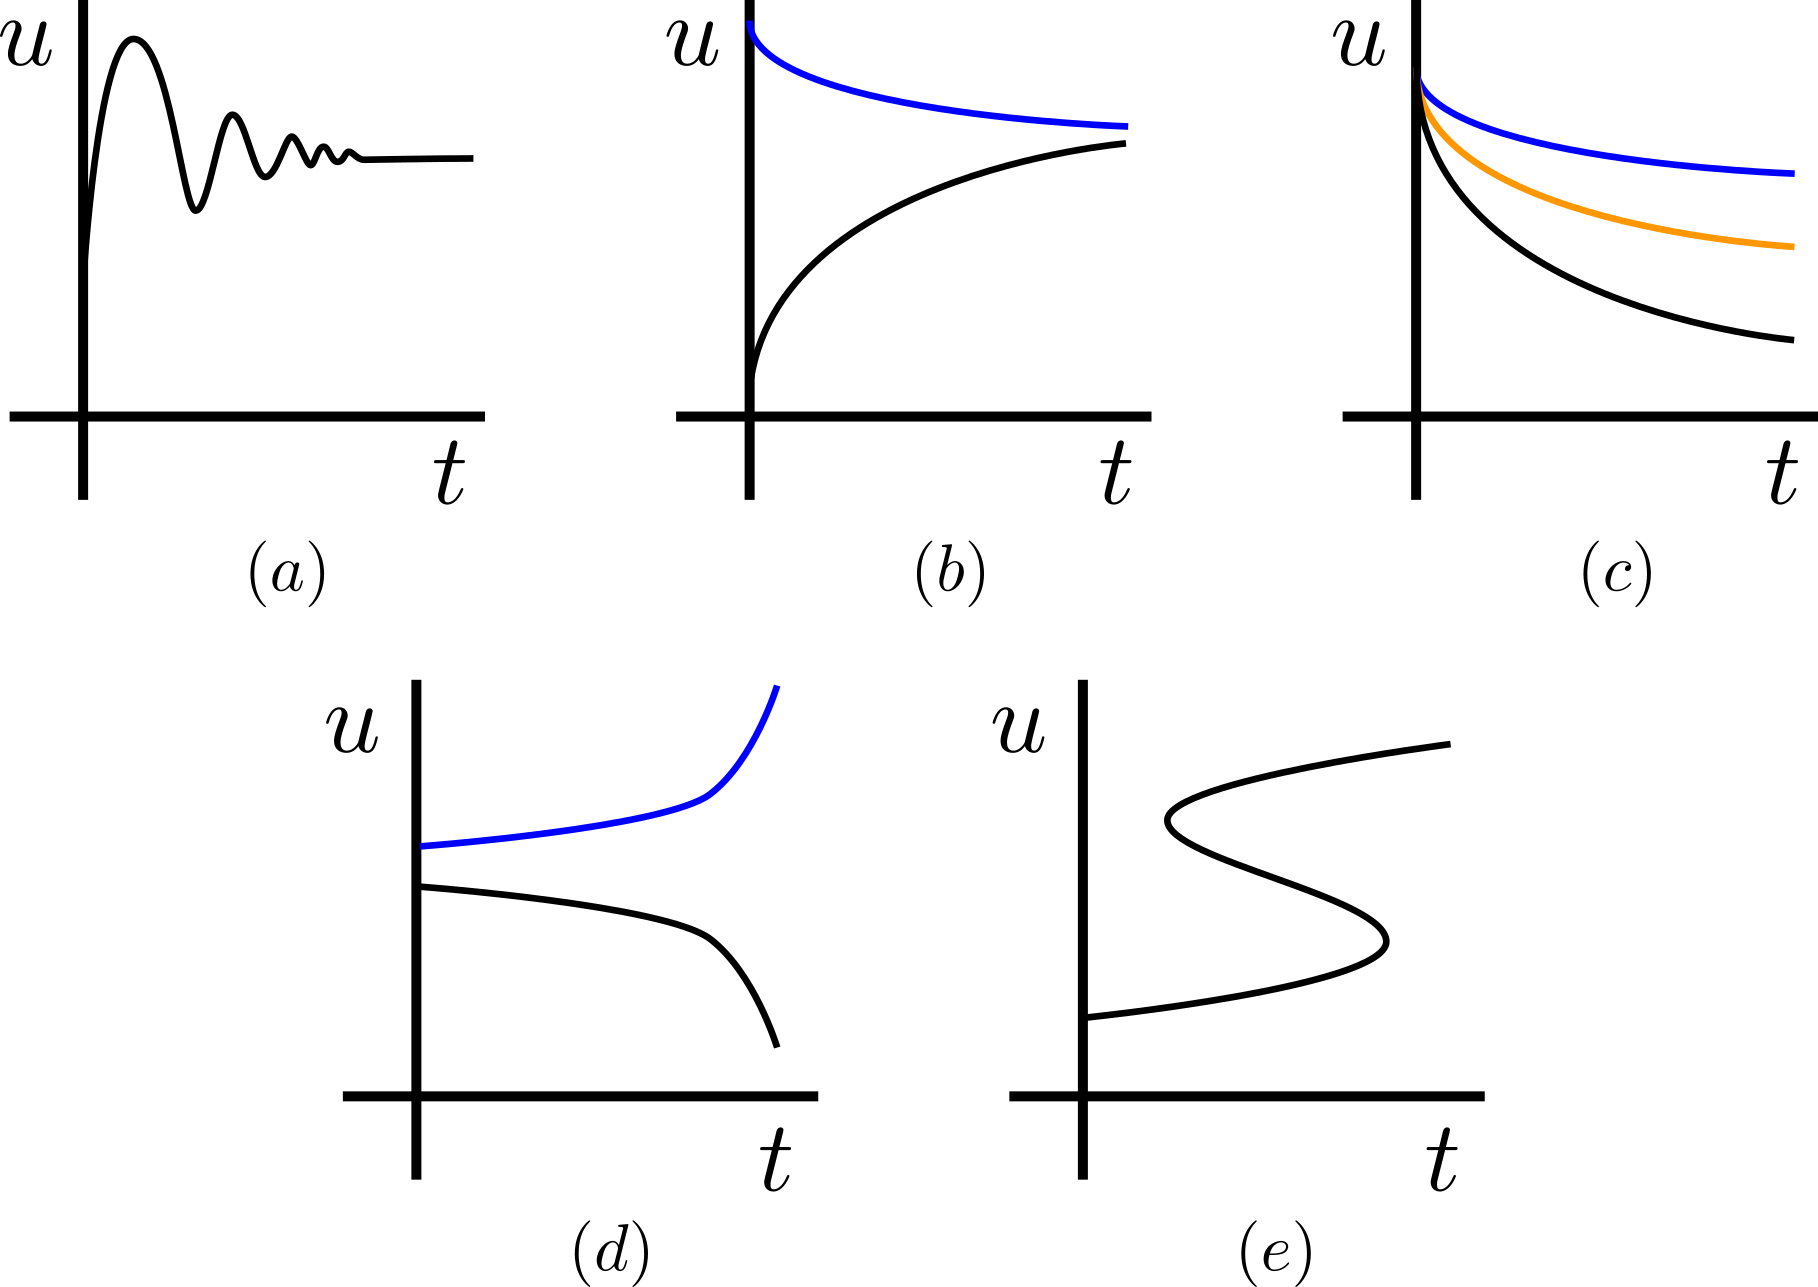
\includegraphics[width=0.7\textwidth]{../../Pictures/Possible_trajectories.png}
\caption{\label{Possible_trajectories} Which sketches could arise from a set of ODEs?}
\end{figure}
\begin{Answ}
\subsection{Answers}
\begin{enumerate}[(a)]
\item Non-monotonic, thus, cannot be produced by a single autonomous equation. A system of autonomous equations could produce the sketch.
\item Top trajectory is strictly monotonically decreasing, the bottom trajectory is strictly monotonically increasing. This system could be produced by a single autonomous ODE, \eg the logistic equation.
\item All trajectories are strictly monotonically decreasing. The trajectories cannot be produced by an autonomous ODE system as we have non-uniqueness. Namely, all trajectories as the same initial condition.
\item Top trajectory is strictly monotonically increasing, the bottom trajectory is strictly monotonically decreasing. This system could be produced by a single autonomous ODE.
\item The curve is not well-defined, namely it is not singular valued for time, thus, it is non-monotonic and cannot be produced by an ODE system.
\end{enumerate}
\end{Answ}
\section{Taylor expansion}
No, not even I can make these interesting. Practice your expansion skills, it is good for your (mathematical) health. Expand each of the following functions about $x=0$ to quadratic order \ie
\bb
\exp(x)\approx 1+x+\frac{1}{2}x^2.
\ee
\begin{enumerate}
\item $\cos(x)$.
\item $\frac{1}{1-x}$.
\item $\cos(x)\cos(y)-\sin(x)\sin(y)$.
\end{enumerate}
Finally, expand 
\bb
\frac{x}{1-x-x^2}
\ee
to sixth order about zero. What is interesting about the coefficients of the powers of $x$?
\begin{Answ}
\subsection{Answers}
\begin{enumerate}
\item $1-{\frac {1}{2}}{x}^{2}$.
\item $1+x+{x}^{2}$.
\item $1-1/2\,{y}^{2}-1/2\,{x}^{2}-xy$.
\item $x+{x}^{2}+2\,{x}^{3}+3\,{x}^{4}+5\,{x}^{5}+8\,{x}^{6}$.
\end{enumerate}
The coefficients of the last sequence are the Fibonacci sequence.
\end{Answ}
\section{Computer simulation}
I will be putting a simulation problem on each question sheet to help get you gain some coding skills. We will build up the skills slowly so you do not have to worry about being dropped in at the deep end.

If you feel you are ready for a more advanced challenge then all codes in the course are available to modify, have fun.

Finally, all of my codes are written using MatLab's programming language. If you feel more comfortable in Maple, Mathematica, Python, etc. then please feel free to code the problem up using your own abilities.
\subsection*{Three body problem}
Open up the function  at the top of the code you will see the lines

%\lstinputlisting{../Matlab/Three_body_problem.m}
\begin{ttfamily}
m1=1;m2=1;m3=1; \% Masses

G=1; \% Gravitational constant

r10=1;r20=-1;r30=1i; \% Initial positions

v10=1i*0.5;v20=-1i*0.5;v30=1i*0.5; \% Initial velocities
\end{ttfamily}


These are the parameters of the code. Currently: all masses are equal to 1; the gravitational coefficient is 1; the initial positions of the masses is (1,0), (-1,0) and (0,1); and the initial velocities are (0,1/2), (0,-1/2) and (0,1/2). Note that the code is written using complex variables as Cartesian coordinates \ie $(x,y)$ is written $x+Iy$, or \texttt{x+1i*y} in MatLab.

\begin{enumerate}
\item Have a play around with the parameters and watch chaos unfurl before you eyes.
\item Can you find parameters that will create an orbiting solar system? Hint: Make one mass really large and the others small (\ie \texttt{m1=1000, m2=0.01, m3=0.01}). Place the first mass at the origin, the second at (10,0) and the third at (20,0) (\ie \texttt{r10=0, r20=10, r30=20}). Now play with the velocities to try and cause the masses \texttt{m2} and \texttt{m3} to orbit \texttt{m1} \see{TBP_orbits}.
\item Can you find an initial set of positions and velocities that will allow all three bodies to orbit each other in a circle \see{TBP_circle}?
Hint: Symmetry is key to this question. All masses must be the same. Place the masses initially on the points of an equilateral triangle. Play with the velocities to try and cause the masses to move in a circle.
\end{enumerate}
\begin{figure}[h!!!tb]
\centering
\subfigure[\label{TBP_orbits}]{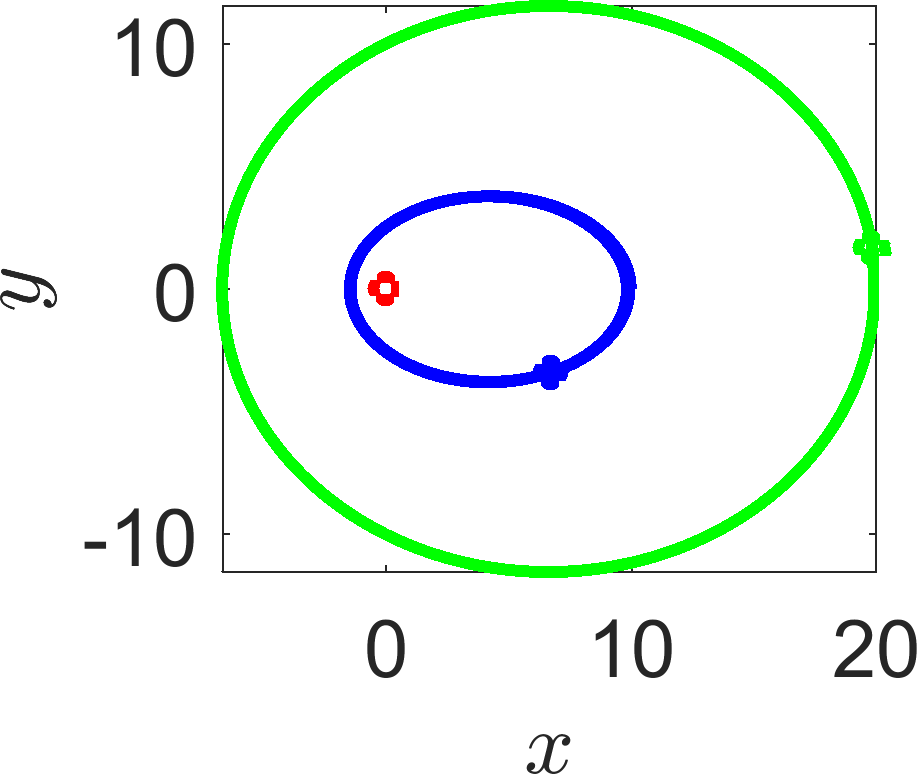
\includegraphics[height=\tttp]{../../Pictures/TBP_orbits.png}}
\subfigure[\label{TBP_circle}]{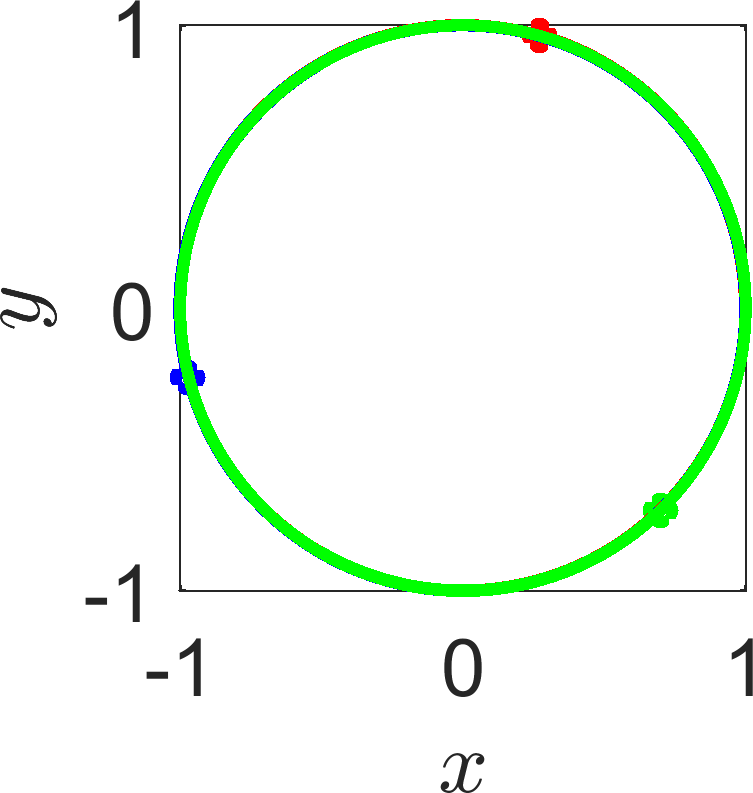
\includegraphics[height=\tttp]{../../Pictures/TBP_circle.png}}
\caption{\label{Two_body_problem} (a) An orbiting system. (b) Planets chasing one another.}
\end{figure}
\begin{Answ}
\subsection{Answers}
\subsubsection{}
Students should be able to offer interesting parameter combinations.
\subsubsection{}
Let the initial velocities be \texttt{v10=0;v20=1i*5;v30=1i*5;} and you'll get nice elliptic orbits.
\subsubsection{}
The key to this question is to note that the velocity must be tangent to the circle on which the masses are moving. Further, we can simplify our job by writing position and velocities in complex variables. Namely

\begin{ttfamily}
rr=0.76;\% Radius of circle

r10=1;r20=exp(1i*2*pi/3);r30=exp(1i*4*pi/3);


v10=rr*exp(1i*pi/2);v20=rr*exp(1i*2*pi/3+1i*pi/2);v30=rr*exp(1i*4*pi/3+1i*pi/2);
\end{ttfamily}
\end{Answ}
\section*{Exam Revision}
Here are a some of questions that are along the same lines as the above that can be saved for exam revision.
\section{Drag racing}
In order for an object to move over a flat surface the applied horizontal force required to push the object must overcome the friction between the object and the surface. The friction force is proportional to the object's weight,
\bb
F=-\mu mg.
\ee
Since the entire force pushing a dragster forward is due to friction (between the tires and the road), we expect the maximum force propelling the dragster forward will be when $\mu=1$.
\begin{enumerate}
\item Use Newton's second law of motion, (Force=mass$\times$acceleration, or $F=m\ddot{x}$) to calculate the time a drag racer would take to complete a standard quarter-mile
course (402.34 meters).
\item On June 2, 2001, Kenny Bernstein set the world record for a
quarter mile track with a time $t = 4.477$ seconds. What assumptions have we made that causes to over estimate this time?
\end{enumerate}
\begin{Answ}
\subsection{Answers}
\subsubsection{}
Solving Newtons Second Law we get
\bb
x(t)=gt^2/2.
\ee
Substituting in the known values
\bb
\sqrt{402.34\times 2/9.81}= 9.1 \textrm{s}.
\ee
\subsubsection{}
We assumed that the maximum force on the vehicle would be $mg$, however, initially the tires of a dragster will adhere more strongly to the racing surface so that they can ``push off''. This means that initially $\mu>1$. Applying more force to the road means that the car accelerates faster than expected.
\end{Answ}


\section{Newton's law of cooling}
\bb
\dot{T}=k(T_\infty-T)\label{Newtons_law_cooling}.
\ee
You can find the temperature inside your refrigerator without putting a thermometer inside. Take an item out of the fridge that has had chance to acclimatise to the temperature inside the fridge. For example, a can of fizzy drink would be perfect. Let the can warm for one minute and take its temperature. Let it warm for another minute and record its temperature again.

Suppose that the readings are $T(1) = 5\degree$C and $T(2)=8\degree$C and that the ambient temperature is 17$\degree$C.

\begin{enumerate}
\item What is the temperature inside the fridge?
\item Measurement are prone to error. Suppose your first and second measurements have an error of $\pm10\%$. Namely, the first measurement could be anywhere in the range [4.5,5.5]$\degree$C and similarly the second measurement could be anywhere in the range [7.2,8.8]$\degree$C. What are the possible maximum and minimum temperatures inside the fridge?
\item Why would it be problematic if we left measured the second temperature after a much longer time?
\end{enumerate}
\begin{Answ}
\subsection{Answer}
\subsubsection{}
Solve \eqn{Newtons_law_cooling},
\bb
\dot{\l e^{kt}T\r}=kT_\infty e^{kt},
\ee
\bb
\implies T=T_\infty+Ce^{-kt}.
\ee
Substitute in the known information:
\begin{align}
5&=17 +Ce^{-k},8=17+Ce^{-2k},\\
\implies -12&= Ce^{-k},-9=Ce^{-2k}.\label{Rearranged}
\end{align}
Square the first equation of \eqref{Rearranged} and divide by the second equation \eqn{Rearranged},
\bb
\frac{12^2}{-9}=\frac{C^2e^{-2k}}{Ce^{-2k}}.
\ee
Hence, $C=-16$. We could work out $k$ as well, but we do not need it since, we want to know $T(0)=T_\infty+C=17-16=1\degree$C.

\subsubsection{}
We essentially rerun the above analysis but with unknown temperatures $T_1$ and $T_2$. Specifically,
\bb
\frac{\l T_1-17\r^2}{T_2-17}=C.\label{C}
\ee
The largest $C$ can be is when $T_1$ is as far away from 17$\degree$C as possible, \ie 4.5$\degree$C, and $T_2$ is as close possible, \ie 8.8$\degree$C. Thus, $T(0)=17+\l 4.5-17\r^2/\l 8.8-17\r\approx-2.1$. Similarly, the smallest $C$ be will is when $T_1$ and $T_2$ take the opposite limits of there intervals $T(0)=17+\l 5.5-17\r^2/\l 7.6-17\r\approx3.5\degree$C.
\subsubsection{}
Measuring $T(0)$ relies on measuring $C$, which, in turn, relies on measuring the denominator of \eqn{C}. The greatest error in $C$ will appear when $T_2\approx17\degree$C because small changes in $T_2$ will lead to large changes in $C$. Since $T(t)\rightarrow 17$ as $t\rightarrow\infty$, then larger errors will appear if we measure the second temperature too far into the future.
\end{Answ}
\section{More Taylor}
Expand to quadratic order
\begin{enumerate}
\item $\sin(x)$.
\item $\cos(\sin(x))$.
\item $\sin(\cos(x))$.
\item $1/\cos(x+y)$.
\end{enumerate}
\begin{Answ}
\subsection{Answer}
\begin{enumerate}
\item $x$.
\item $1-\frac{x^2}{2}$.
\item $\sin(1)-\frac{1}{2}\cos(1)x^2$.
\item $1+\frac{1}{2}x^2+yx+\frac{1}{2}y^2$.
\end{enumerate}
\end{Answ}
%Solution:
%Taking the time one half hour after the soda was removed from
%the refrigerator to be the ìzero timeî(and stating the given information in
%an appropriate way), we have the boundary value problem
%dT
%dt
%=
%k
%(70
%
%
%
%
%
%
%\item \textbf{Logistic equation}
%\begin{align}
%\frac{\rd u}{\rd t}&=rcu\l 1-\frac{u}{c}\r,\nonumber\\
%\Rightarrow\int_0^T\frac{\rd u}{u(1-u/c)}&=\int_0^Trc \rd t,\nonumber\\
%\Rightarrow\int_0^T \frac{1}{u}+\frac{1/c}{1-u/c}  \rd u&=rcT,\nonumber\\
%\Rightarrow\left[\ln(u)-\ln\l 1- \frac{u}{c} \r \right]^T_0&=rcT,\nonumber\\
%\Rightarrow\ln\l\frac{u}{1- \frac{u}{c}} \r-\ln\l\frac{u_0}{1- \frac{u_0}{c}} \r&=rcT,\nonumber\\
%\Rightarrow u(T)=\frac{c}{1+\frac{c-u_0}{u_0}\exp\l{-rcT}\r}
%\end{align}
%
%\item \textbf{Bacteria growth}
%\dot{u}=v
%\dot{v}=-uv
%
%\item \textbf{Time shift in ODEs, arbitrary start point}
%\item \textbf{Taylor series}
%\item \textbf{Wobbling doors} Damped oscillator.
%
%\item \textbf{Two body problem}
%We can combine the Second Law of Motion and the Law of Gravitation in order to predict the position of planets interacting through their gravitational fields \see{Two_body}. Consider two planets with the same mass, $m$, and positions $\bm{r}(t)_1$ and $\bm{r}(t)_2$, respectively. Further, we note that since we are dealing with acceleration (a second order equation) we will need to specify two initial conditions, the position and velocity. Let the initial positions be $\bm{r}(0)_1=\bm{r}_{10}$ and $\bm{r}(0)_2=\bm{r}_{20}$ and the initial velocities $\dot{\bm{r}(0)_1}=\bm{v}_{10}$ and $\dot{\bm{r}(0)_2}=\bm{v}_{20}$. The governing equations are
%\begin{align}
%&m\ddot{\bm{r}_1}=-G\frac{m^2}{|\bm{r}_1-\bm{r}_2|^3}\l\bm{r}_1-\bm{r}_2\r,\label{g1}\\
%&m\ddot{\bm{r}_2}=-G\frac{m^2}{|\bm{r}_2-\bm{r}_1|^3}\l\bm{r}_2-\bm{r}_1\r\label{g2}.
%\end{align}
%where we remember that this is a vector equation, $\bm{r}_i=(x_i,y_i)$, so there are actually four ODEs here, rather than two.
%
%We notice that if we add the equations together the right-hand sides cancel out,
%\bb
%\ddot{\bm{r}_1}+\ddot{\bm{r}_2}=0.
%\ee
%Integrating this equation we find that the velocity of $\bm{r}_1+\bm{r}_2$ is a conserved quantity and that
%\bb
%\bm{r}_1+\bm{r}_2=(\bm{r}_{10}+\bm{r}_{20})+(\bm{v}_{10}+\bm{v}_{20})t.\label{COM}
%\ee
%Points to note:
%\begin{itemize}
%\item the defined quantity $\bm{R}=(\bm{r}_1+\bm{r}_2)/2$ is the centre of mass of the system (because $m_1=m_2$). Thus the motion of the two planets is constrained such that their centre of mass travels at a constant speed throughout space;
%\item using \eqn{COM} we could decouple \eqns{g1}{g2} into two separate non-autonomous ODEs;
%\item it turns out to be more fruitful to consider the quantity $\bm{r}_1-\bm{r}_2$, which, if written in polar coordinates, leads to an ODE with a closed form solution. We will not do this here, but we will consider the simulated results.
%\item when solving \eqns{g1}{g2} numerically we could separate each equation into its Cartesian components and reduce the second order equation to two first order equations. Namely, we introduce $(v_{ix},v_{iy})=(\dot{x}_i,\dot{y}_i)$. Thus, we would have a system of eight ODEs to solve, with variables $(x_1,y_1,v_{1x},v_{1y},x_2,y_2,v_{2x},v_{2y})$. However, since $x_i$ and $y_i$ are perpendicular Cartesian coordinates it turns out to be a good idea to use complex numbers. Specifically, instead of writing two ODEs for each of $x_i$ and $y_i$ we can simply solve one ODE in terms of the complex quantity $\bm{r}_i=x_i+Iy_i$, which can be handled by numerical solvers. Thus, we simplify the numerical solution from eight equations to four equations.
%\end{itemize}
\end{document}